\section{Problem Definition}
\label{sec:problem_definition}

In order to define the problem of stale transaction categories we must first discuss the problem of concurrent database transactions in a web service environment.

In traditional database systems, transactions are executed with \gls{acid} properties to ensure correctness, durability, and consistency among all transactions that are executed on the system. When transactions are moved to a web service context where concurrent transactions occur frequently, the traditional model of transaction correctness is not feasible to deploy. Multiple interleaving transactions with the locking required in \gls{acid} systems causes an overhead that is not acceptable for the end user. In order to accommodate concurrent transactions in a web service environment that execute in an acceptable time frame, locking is removed and transactions are allowed to execute and commit independently. While all transactions are executing and committing successfully then there are no solutions and the lack of locks works. However, in the event that a transaction fails and there are transactions that are dependent downstream then a cascading rollback occurs reverting the effects of the downstream transaction. All transactions are put on hold until a compensation transaction, generated by the scheduler to fix the results of the failed transaction, can execute successfully. This causes a lot of overhead in the system that can be avoided if the failed transaction can be isolated from dependent transactions.

In our previous work (see \cite{ravan_ensuring_2020}) we presented a prediction-based transaction scheduler that provides appropriate run times for web service environments. The scheduler predicts the outcome of a transaction based on the transactions execution history. The transaction is then placed into one of four categories based on whether commit rate and execution time. We then provided custom locking actions based on the transactional category. Transactions in categories with high commit rates and low execution times are allowed to execute concurrently while transactions in categories with low commit rates and long execution times are locked to prevent downstream effects.

Our previous work addresses the problem of cascading rollbacks and compensation transactions, however a new problem presents itself in a transaction that has been incorrectly categorized or its metrics have changed and it needs to be re-categorized. This becomes a problem when a transaction with a high commit rate is locked due to its category when it can execute concurrently without any undesired side effects. The other extreme and more disastrous use case is a transaction with a low commit rate that should be locked but executes concurrently with other transactions and causes those transactions to abort their executions. In these situations we need the ability to promote or demote a transaction as its execution history changes. 

As we discuss the use of the transaction's execution history, another problem presents itself; what do we do with transactions that are new to the system and do not have any execution history? If we are to address the problem of transactions with no execution history then a reputation score should take the place of the previous four category solution. An objective reputation score allows for a linear approach for transaction comparisons that provides two benefits; a more granular comparison (i.e. comparing transactions that would normally be within the same category and would previously conflict) and a default score for a transaction with no history. In the previous four category solution, there is no default category for transactions with no history. 

In our previous solution, we defined three different locking actions; grant (+), decline (-), and elevate ($\delta$). The decline action causes a transaction to wait for resources to become available. Due to the restrictive four categories of our previous solution, there are a large number of scenarios where a decline action would occur. By transitioning to a solution that is more granular, we could potentially turn decline actions into elevate actions. The elevate action will abort a transaction of a lower category in order for a transaction of a higher category to be granted access to needed resources. By design this prevents transactions that are well-behaving from being hindered by transactions that are not well-behaving. However, if we don't include the cost of an aborted transaction in our calculation then we could do more harm than good by elevating too frequently. Transitioning to a new metric will allow us too refine our rules for elevation to prevent elevate actions that cause more harm than benefit. See Tables \ref{tbl:read_lock_compatibility} and \ref{tbl:write_lock_compatibility} for reference. In the next section we walk through an airline ticketing use-case scenario to better explain the problems identified.

% This situation assumes that not only can the transaction be categorized but it can also be identified from other transactions executing in the system. Transaction identification will allow for a transaction to be identified from other transactions in the system and provide a uniqueness that can be pinpointed. This also shows that the transaction's execution should be translated into an objective reputation metric that can be scored as the execution history grows. 

\subsection{Use-Case Scenario}
\label{subsec:use_case_scenario}

In order to better explain the problems, let's look at a use case scenario of an airline ticketing system. Let's say we have two users that are attempting to reserve seats on an airline. The first user places a ticket, or a seat, in their shopping cart using an airline's online reservation system. While in the shopping cart, that seat is no longer available for reservation even though the transaction has not been completed. Simultaneously, a second user attempts to reserve a seat on the same airline and same flight. There are no seats available so that user is denied a reservation. Later on, the first user that placed the initial reservation in their shopping cart does not purchase the reservation in time. Their reservation is then expired and made available again.

In this scenario, the seat is made available due to the reconciliation efforts of the reservation system, however, in the end the airline loses profit. A seat that could have been purchased by the second user was not available due to the first user having placed the seat in their shopping cart. See the scenario diagram in Figure \ref{image:airline_reservation}. Figure \ref{image:airline_reservation_system_model} shows the same scenario with the transaction scheduler and database contained within the same logical unit. In both figures the solid lines represent the user transactions submitted to the database while the dotted lines represent the response from the transaction. The gray swim lanes labeled $T_0$, $T_1$, and $T_2$ show the transactions at certain time intervals.

\begin{figure}
\centering
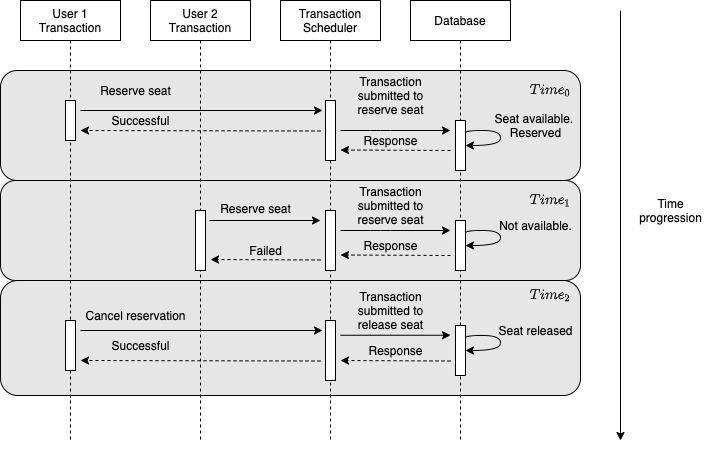
\includegraphics[scale=0.50]{images/AirlineReservation.png}
\caption{Airline Reservation Use Case}
\label{image:airline_reservation}
\end{figure}

\begin{figure}
\centering
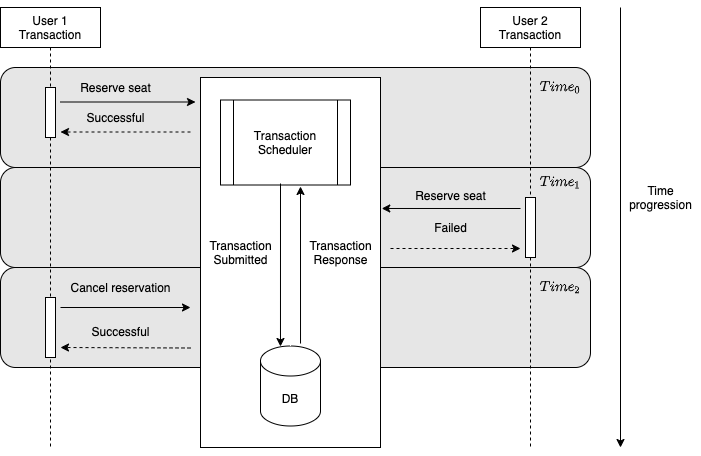
\includegraphics[scale=0.50]{images/AirlineReservation_Overview.png}
\caption{Airline Reservation Use Case System Model}
\label{image:airline_reservation_system_model}
\end{figure}

If the given scenario were to play out in a system that maintained the reputation of transactions entering the system, then the behavior of the first user would be tracked would be taken into consideration. The next time the user were to submit a similar transaction, that reputation would be taken into consideration and could potentially prevent the user from getting precedence over the seat reservation. This reinforces good user behavior in the system and also increases profit for the reservation system. In the next section, we discuss the related work that influenced the current problem and research.